\chapter{Deskripsi Solusi}

Pada bab ini dituliskan analisis terkait kebutuhan sistem pada KodeBareng, masalah pada implementasi ILE yang sudah ada, serta ragam solusi yang dapat diimplementasikan.

\section{Analisis Masalah}
KodeBareng adalah platform berbasis web sebagai sarana pembelajaran pemrograman menggunakan gamifikasi. Pada platform ini, dibutuhkan suatu \textit{interactive learning environment} (ILE) yang dapat mendukung aktivitas pemrograman secara praktis. ILE diharapkan dapat meningkatkan kemampuan pemecahan masalah dan implementasi kode penggunanya dengan adanya wadah menulis dan menjalankan kode secara daring. ILE dibangun secara modular pada platform KodeBareng sehingga tidak terlalu disruptif terhadap sistem yang sudah ada.

% Dalam beberapa sistem yang sudah ada seperti \href{https://olympia.id/}{Olympia}, ILE yang dapat menjawab kebutuhan ini biasanya berupa sistem submisi kode implementasi yang menggunakan autograder untuk penilaiannya. Sayangnya, hal ini dinilai kurang interaktif karena setiap perubahan kode yang dilakukan pengguna harus melakukan submisi ulang dan menjalankan kembali programnya. Pengguna juga menjadi tidak tahu kesalahannya dimana, serta masih harus dapat menjalankan kodenya secara manual di mesinnya.

Pada beberapa platform lain seperti yang sudah dibahas pada bab sebelumnya, terdapat berbagai macam jenis ILE yang masing-masing memiliki kelebihan dan kekurangannya masing-masing. ILE visual seperti yang digunakan pada \textcite{brilliant2021media} memiliki interaktivitas yang sangat tinggi dan mudah dipahami, namun kurang dapat diimplementasikan secara umum dan tidak langsung menyentuh implementasi kode. Sementara itu, terdapat juga ILE yang berupa Web IDE namun kebanyakan implementasinya hanya sebatas eksekusi kode pada wadah teks yang diberikan. Keterbatasan ini membuat proses pembelajaran terhambat akibat kurangnya ada pembantu yang dapat digunakan oleh pengguna untuk mencari letak kesalahan dalam implementasi kodenya, serta menjadikan Web IDE terlalu menantang bagi pemula yang ingin belajar pemrograman.

% REVISI II
% KodeBareng adalah platform berbasis web sebagai sarana pembelajaran pemrograman menggunakan gamifikasi. Metode pembelajarannya berbasis teks, visual interaktif, serta kuis-kuis. Kuis-kuis tersebut dapat berupa pilihan ganda, isian singkat, ataupun pencocokan jawaban yang membahas materi terkait yang sudah dipelajari. Dengan adanya kuis tersebut, diharapkan pelajar tidak hanya bisa memahami teori namun juga implementasi kode dari teori yang telah dijabarkan, seperti dengan adanya pertanyaan terkait hasil keluaran suatu kode. Namun, pertanyaan kuis semacam itu memiliki limitasi karena pelajar tidak dapat membuat sendiri implementasi kode sehingga susah untuk mengukur pemahaman praktis dan kemampuan pemecahan masalah menggunakan teori yang telah diberikan. Padahal, pemrograman adalah suatu kemampuan yang membutuhkan banyak latihan praktik implementasi agar pemahaman dapat tercapai secara optimal.

% Alternatif lain juga bisa dengan memberikan permasalahan yang harus dipecahkan kemudian pelajar dapat mengimplementasikan sendiri terlebih dahulu di mesinnya lalu melakukan submisi kode pada platform. Hal ini menimbulkan permasalahan lain seperti susahnya melakukan pemecahan permasalahan pada instalasi spesifik mesin yang digunakan oleh pelajar, adanya perbedaan versi dari lingkungan mesin pelajar dan mesin penguji yang dapat menimbulkan masalah dalam pengetesan, dan juga membuat platform lebih terbatas portabilitasnya karena instalasi hanya terbatas pada mesin dan lingkungan sistem tertentu. Permasalahan lain juga timbul dari cara melakukan penilaian dan pengetesan kode yang telah dibuat, karena apabila dilakukan secara manual akan membutuhkan banyak tenaga kerja.

% REVISI I
% Saat ini, terdapat banyak sekali metode penyampaian materi pembelajaran pemrograman secara daring. Namun, agar dapat memvalidasi pengetahuan yang didapat diperlukan sistem pendukung yang dapat digunakan sebagai media praktik bagi para pelajar. Kurangnya praktik dan latihan dalam pembelajaran dapat membuat adanya pemisah antara pemahaman teori dan praktik. (\textit{!TODO: ceritakan paper mengenai ini})

% Untuk memvalidasi pengetahuan yang sudah dipelajari, terdapat banyak metode yang dapat digunakan. Salah satu metode yang sering dipakai adalah kuis yaitu serangkaian pertanyaan yang mengacu pada materi yang telah diberikan. Kuis dapat dibuat dalam berbagai macam bentuk seperti pilihan ganda, isian singkat, esai, dll. Metode esai dapat digunakan untuk memvalidasi logika dan pola pikir dari pemecahan masalah, namun karena esai tersebut merupakan kode maka harus terdapat sistem yang dapat mengeksekusi, menilai, serta memberikan \textit{feedback} dari hasil eksekusi kode tersebut layaknya pemrograman yang sebenarnya.

% Maka dari itu, diperlukan sistem pembelajaran pemrograman interaktif yang dapat dipakai pengguna untuk menuliskan kode, memberikan \textit{feedback} dari kode yang dibuat, serta menilai kebenaran dari kode tersebut. \textit{Feedback} yang diberikan berupa hasil eksekusi kode berupa pesan keluaran apabila kode berhasil dijalankan, serta pesan error apabila terjadi masalah dalam eksekusi kode. Pesan keluaran hasil eksekusi dapat dibandingkan dengan pesan keluaran yang seharusnya agar dapat dinilai dan diberitahukan kepada pengguna sehingga pengguna dapat mengetahui letak kesalahan dari kode yang diimplementasikan.

\section{Analisis Solusi}
Berdasarkan studi literatur terhadap beberapa platform pembelajaran lainnya, metode pembelajaran pemrograman dapat dikategorikan menjadi visual dan non-visual. Metode pembelajaran pemrograman yang visual tidak langsung menggunakan kode seperti pada \textcite{brilliant2021media}, tetapi menggunakan perumpaan visual yang interaktif dengan memakai gambar, simbol, serta animasi. Metode ini membuat pembelajaran menjadi lebih menarik dan mudah, karena diekspresikan dalam bentuk visual. Namun, metode ini tidak menyentuh secara langsung aktivitas pemrograman secara praktis sehingga ada kemungkinan dapat terjadi perbedaan antara teori dan praktik yang dipahami pelajar dengan implementasi program yang sebenarnya. Metode ini juga memiliki bentuk yang spesifik terhadap konten materi yang dibawa, sehingga tidak dapat dipakai untuk konten materi lainnya. \textcite{froggy2021media} juga termasuk pada kategori ini, karena implementasinya hanya spesifik pada materi yang dibawa, khususnya pada materi pengembangan web.

Metode non-visual kebanyakan menggunakan Web IDE dalam pembelajarannya. Pengguna dapat berinteraksi dengan Web IDE sehingga mereka dapat melatih kemampuan pemecahan masalah dan pemrograman praktis. Web IDE yang digunakan biasanya memiliki kapabilitas untuk mengembalikan hasil keluaran dari eksekusi kode, serta melakukan penilaian terhadap kebenaran implementasi. Web IDE juga dapat menerima berbagai macam bahasa sesuai dengan kebutuhan materi yang sedang dipelajari. Selain itu, terdapat juga Web IDE yang menyimulasikan terminal ketimbang editor kode seperti yang dapat dilihat di Katacoda \parencite{katacoda2021media}. Selain itu, Web IDE bisa dikembangkan lebih lanjut pada aspek kolaboratif \parencite{tran2013interactive} ataupun mendukung visualisasi langkah eksekusi program seperti pada \textcite{guo2013pythontutor}. Visualisasi langkah eksekusi menjadi salah satu aspek yang menarik karena tidak banyak ditemukan implementasinya pada platform pembelajaran pemrograman yang sudah terkenal.

\section{Rancangan Solusi}
Dalam makalah ini, dibuat prototipe ILE yang terdiri dari beberapa komponen yaitu Web IDE pada \textit{frontend} dan sistem eksekutor kode pada \textit{backend} yang terpisah dari \textit{backend} KodeBareng.

\begin{figure}[H]
  \centering
  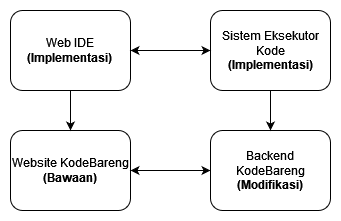
\includegraphics[width=0.5\textwidth]{chapter3/diagramblok.png}
  \caption{Rancangan Solusi ILE}
\end{figure}

Keterangan gambar:
\begin{itemize}
  \setlength\itemsep{-0.2cm}
  \item Implementasi: Komponen diimplementasikan dari awal hingga akhir.
  \item Modifikasi: Komponen hanya perlu diubah beberapa bagian.
  \item Bawaan: Komponen tidak berubah.
\end{itemize}

Pada \textit{frontend}, akan dibuat komponen Web IDE berupa editor kode yang dapat menerima masukan kode serta memberikan \textit{basic syntax highlighting}. Web IDE dapat menampilkan hasil keluaran ataupun kesalahan eksekusi yang dikembalikan dari \textit{backend}, serta hasil penilaian dari pengetesan kode. Web IDE juga dapat menampilkan visualisasi langkah jalannya program agar dapat memudahkan proses pembelajaran dan pencarian letak masalah dalam implementasi kode.

Pada \textit{backend}, akan dibuat sistem eksekutor kode yang terhubung ke backend KodeBareng. Sistem ini menerima kode dan informasi lainnya dari \textit{backend} lalu melakukan eksekusi kode yang akan dinilai berdasarkan hasil keluarannya. Sistem ini juga dapat terhubung pada \textit{backend} KodeBareng apabila dibutuhkan integrasi lain di kemudian hari.